\chapter{MATLAB}\label{ch:appAlabel}
\section{Waveform, FFT and spectrogram script}
\begin{lstlisting}[language=Matlab, flexiblecolumns=true, caption = MATLAB script.]
%------------------------------------------------
%Loading the "Hello" sample
subplot(3,1,1);
[y,Fs] = audioread('microphone-results.wav');
sound(y,Fs);
    dt = 1/Fs;
    t = 0:dt:(length(y)*dt)-dt;
    %figure();
    plot(t,y); xlabel('Seconds'); ylabel('Amplitude');
title('Hello waveform');
%------------------------------------------------
%Creating the FFT of the signal
subplot(3,1,2);
N = length(y);
NEFT = 2^nextpow2(N)
Xk=fft(y, NEFT)/N; % perform N-point DFT of signal
fa = 8000/2*linspace(0,1,NEFT/2+1); 
%figure();
plot(fa, 2*abs(Xk(1:NEFT/2+1)));
title('FFT Spectrum Estimates / Power Spectral Density');
xlabel('Frequency Index'),
ylabel('Amplitude');
%------------------------------------------------
% Creating the Spectrogram
%figure();
subplot(3,1,3);
s = spectrogram(y);
spectrogram(y,'yaxis')
%------------------------------------------------
\end{lstlisting}

\begin{figure}[H]
	\centering
	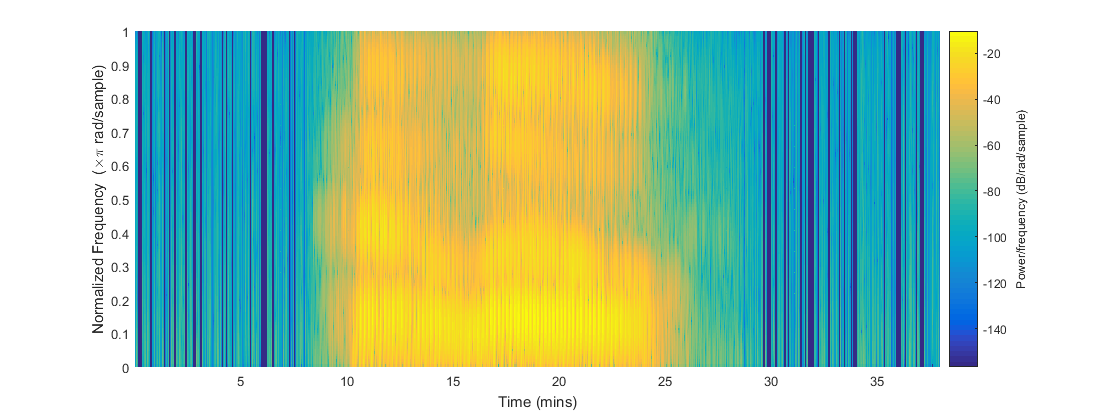
\includegraphics[width=\textwidth]		
	{speech_processing/04_Spectrogram}
	\caption{Spectrogram generated from FFT.}
	\label{fig:Spectrogram}
\end{figure}








